%% -*- coding:utf-8 -*-
\section{Monoidal object}

Monoid plays very important role in category theory

\section{Monoid in $\cat{Set}$}
Lets consider \mynameref{def:monoid} in the terms of Set theory and
will try to give the definition that is based rather on morphisms then
on internal set structure. Consider a set $M$ and by the definition
$\forall m_1, m_2 \in M$ we can define a new element of the set
$\mu(m_1, m_2) \in M$. Later we shall use the following notation for
the $\mu$:
\[
\mu(m_1, m_2) \equiv m_1 \cdot m_2.
\]
If the $(M, \cdot)$ is monoid then the following 2 conditions have to
be satisfied. The first one (associativity) declares that $\forall
m_1, m_2, m_3 \in M$ 
\[
m_1 \cdot ( m_2 \cdot m_3) = ( m_1 \cdot
m_2 ) \cdot m_3.
\]
The second one (identity presence) says that
\(
\exists e \in M
\) such that $\forall m \in M$:
\begin{equation}
m \cdot e = e \cdot m = m.
\label{eq:monoid2}
\end{equation}

Lets start with the first one we can define $\mu$ as
\mynameref{def:morphism} in the following way $\mu: M\times M \to M$
where $M \times M$ is \mynameref{ex:set_product} in
\mynameref{def:setcategory}. I.e. $M, M \times M \in \catob{Set}$ and
$\mu \in \cathom{Set}$.  Consider another objects of $\cat{Set}$: $A =
M \times \left( M \times M \right)$ and $A' = \left( M \times M \right)
\times M$. They are not the same but there is a trivial
\mynameref{def:isomorphism} between them $A \cong_\alpha A'$, where
\[
\alpha(x,(y,z)) = ((x,y),z).
\]
Consider the action of \mynameref{def:product_of_morphisms} 
$\idm{M} \times \mu$ on $A$:
\[
\idm{M} \times \mu \left(x,\left(y,z\right)\right) = 
\left(\idm{M}(x),\mu\left(y,z\right)\right) = 
\left(x, y \cdot z\right) \in M \times M
\]
i.e. $\idm{M} \times \mu: M \times \left( M \times M \right) \to M
\times M$. If we act $\mu$ on the result we shall get:
\begin{eqnarray}
\mu \left(\idm{M} \times \mu \left(x,\left(y,z\right)\right)\right) = 
\left(\idm{M}(x),\mu\left(y,z\right)\right) = 
\nonumber \\
=
\mu\left(x, y \cdot z\right) = x \cdot (y\cdot z) \in M,
\nonumber
\end{eqnarray}
i.e. 
$\mu \circ \left(\idm{M} \times \mu\right): M \times \left( M \times M
\right) \to M$.

For $A'$ we have the following one:
\begin{eqnarray}
\mu\circ\left(\mu \times \idm{M}\right)\left(\left(x,y\right),z\right)
= \mu\left(x \cdot y, z\right) = (x \cdot y) \cdot z.
\nonumber
\end{eqnarray}
Monoid associativity requires 
\[
x \cdot (y\cdot z) = 
(x \cdot y) \cdot z
\]
i.e. the morphisms the corresponding morphisms commute:
\[
\mu\circ\left(\mu \times \idm{M}\right) =
\mu \circ \left(\idm{M} \times \mu\right) \circ \alpha.
\]
This corresponds the diagram is at \cref{fig:monoid_mu_alpha}.

\begin{figure}
  \centering
  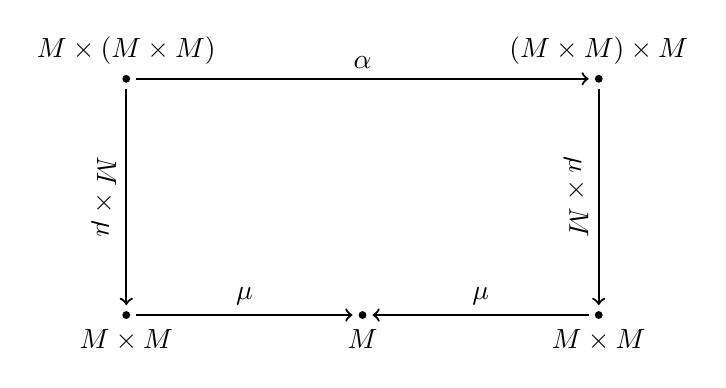
\begin{tikzpicture}[ele/.style={fill=black,circle,minimum
        width=.8pt,inner sep=1pt},every fit/.style={ellipse,draw,inner
        sep=-2pt}]

    % the texts
    
    \node[ele,label=above:$M\times\left(M \times M\right)$] (M31) at (0,3) {};    
    \node[ele,label=above:$\left(M \times M\right)\times M$] (M32) at (6,3) {};    
    \node[ele,label=below:$M \times M$] (M21) at (0,0) {};    
    \node[ele,label=below:$M \times M$] (M22) at (6,0) {};    
    \node[ele,label=below:$M$] (M) at (3,0) {};    

    \draw[->,thick,shorten <=2pt,shorten >=2pt] (M31) to
    node[sloped,above]{$\alpha$} (M32);
    \draw[->,thick,shorten <=2pt,shorten >=2pt] (M31) to
    node[sloped,below]{$\idm{M} \times \mu$} (M21);
    \draw[->,thick,shorten <=2pt,shorten >=2pt] (M32) to
    node[sloped,below]{$\mu \times \idm{M}$} (M22);
    \draw[->,thick,shorten <=2pt,shorten >=2pt] (M22) to
    node[sloped,above]{$\mu$} (M);
    \draw[->,thick,shorten <=2pt,shorten >=2pt] (M21) to
    node[sloped,above]{$\mu$} (M);
  \end{tikzpicture}
  \caption{Commutative diagram for $\mu\circ\left(\mu \times
    \idm{M}\right) = \mu \circ \left(\idm{M} \times \mu\right) \circ
    \alpha$.} 
  \label{fig:monoid_mu_alpha}
\end{figure}
Very often the isomorphism $\alpha$ is omitted i.e. 
\[
M\times\left(M \times M\right)
= \left(M \times M\right)\times M = M^3
\]
and the morphism
equality is written as follow
\[
\mu\circ\left(\mu \times \idm{M}\right) =
\mu \circ \left(\idm{M} \times \mu\right)
\]
The corresponding commutative diagram is shown in
\cref{fig:monoid_mu}.
\begin{figure}
  \centering
  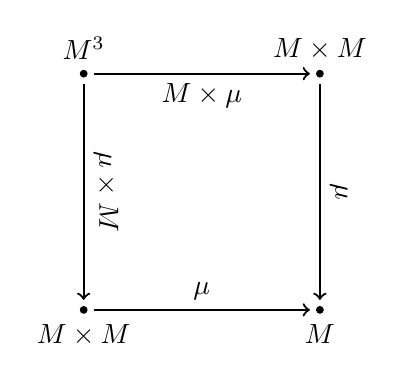
\begin{tikzpicture}[ele/.style={fill=black,circle,minimum
        width=.8pt,inner sep=1pt},every fit/.style={ellipse,draw,inner
        sep=-2pt}]

    % the texts
    
    \node[ele,label=above:$M^3$] (M3) at (0,3) {};    
    \node[ele,label=above:$M \times M$] (M21) at (3,3) {};    
    \node[ele,label=below:$M \times M$] (M22) at (0,0) {};    
    \node[ele,label=below:$M$] (M) at (3,0) {};    

    \draw[->,thick,shorten <=2pt,shorten >=2pt] (M3) to
    node[sloped,below]{$\idm{M} \times \mu$} (M21);
    \draw[->,thick,shorten <=2pt,shorten >=2pt] (M3) to
    node[sloped,above]{$\mu \times \idm{M}$} (M22);
    \draw[->,thick,shorten <=2pt,shorten >=2pt] (M22) to
    node[sloped,above]{$\mu$} (M);
    \draw[->,thick,shorten <=2pt,shorten >=2pt] (M21) to
    node[sloped,above]{$\mu$} (M);
  \end{tikzpicture}
  \caption{Commutative diagram for $\mu\circ\left(\mu \times
    \idm{M}\right) = \mu \circ \left(\idm{M} \times \mu\right)$.}
  \label{fig:monoid_mu}
\end{figure}

For \eqref{eq:monoid2} consider a morphism $\eta$ from
a one point set $I = \{0\}$ to a special element $e \in M$ such that
$\forall m \in M: e \cdot m = m \cdot e = m$. I.e. $\eta: I \to M$ and
$e = \eta(0)$. Consider 2 sets $B = I \times M$ and $B' = M \times I$. 
We have 2 \mynameref{def:isomorphism}s: $B \cong_\lambda M$ and $B'
\cong_\rho M$ where the isomorphisms are defined as follow
\[
\lambda(0, m) = m
\] 
and
\[
\rho(m, 0) = m.
\] 

If we apply \mynameref{def:product_of_morphisms} $\eta \times \mu$ and
$\mu \times \eta$ on $B$ and $B'$ respectively then we get
\begin{eqnarray}
\eta \times \idm{M} \left(0 \times m\right) = e \times m,
\nonumber \\
\idm{M} \times \eta \left(m \times 0\right) = m \times e.
\nonumber
\end{eqnarray}
If we apply $\mu$ on the result then we get
\begin{eqnarray}
\mu \left(\eta \times \idm{M} \left(0 \times m\right) \right) = e \cdot m,
\nonumber \\
\idm{M} \times \eta \left(m \times 0\right) = m \times e.
\nonumber
\end{eqnarray}
\begin{figure}
  \centering
  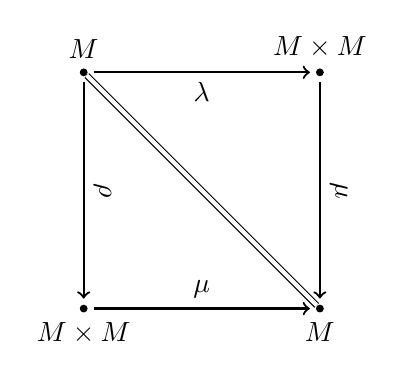
\begin{tikzpicture}[ele/.style={fill=black,circle,minimum
        width=.8pt,inner sep=1pt},every fit/.style={ellipse,draw,inner
        sep=-2pt}]

    % the texts
    
    \node[ele,label=above:$M$] (M') at (0,3) {};    
    \node[ele,label=above:$M \times M$] (M21) at (3,3) {};    
    \node[ele,label=below:$M \times M$] (M22) at (0,0) {};    
    \node[ele,label=below:$M$] (M) at (3,0) {};    

    \draw [double equal sign distance] (M') to (M);
    \draw[->,thick,shorten <=2pt,shorten >=2pt] (M') to
    node[sloped,below]{$\lambda$} (M21);
    \draw[->,thick,shorten <=2pt,shorten >=2pt] (M') to
    node[sloped,above]{$\rho$} (M22);
    \draw[->,thick,shorten <=2pt,shorten >=2pt] (M22) to
    node[sloped,above]{$\mu$} (M);
    \draw[->,thick,shorten <=2pt,shorten >=2pt] (M21) to
    node[sloped,above]{$\mu$} (M);
  \end{tikzpicture}
  \caption{Commutative diagram for $\mu \circ (\eta \times \idm{M})
    \circ \lambda = \mu \circ (\idm{M} \times \mu) \circ \rho =
    \idm{M}$ .} 
  \label{fig:monoid_eta_lambda_rho}
\end{figure}
The \eqref{eq:monoid2} leads to the following equation for morphisms
\[
\mu \circ (\eta \times \idm{M}) \circ \rho = 
\mu \circ (\idm{M} \times \mu) \circ \lambda = 
\idm{M}
\]
or the commutative diagram show on \cref{fig:monoid_eta_lambda_rho}.

\section{Monoidal object}
If we take into consideration that one-point set is
\mynameref{ex:set_terminal_object} then we can conclude that the
monoid can be defined for instance in a \mynameref{def:cartesian_closed_category}
as follow
\begin{definition}[Monoidal object]
\label{def:monoidal_object}
Consider a \mynameref{def:category} $\cat{C}$ with a
\mynameref{def:terminal_object} $t \in \catob{C}$. The object $m \in
\catob{C}$ is called \textit{monoidal object} if the following
conditions satisfied:
\begin{enumerate}
\item the \mynameref{def:product}s $m \times m, m \times t, t \times
  m$ exist 
\item there is a \mynameref{def:morphism} $\mu: m \times m \to m$ in
  the category
\item there is another morphism $\eta: t \to m$
\item the morphisms satisfy the following conditions:
\begin{eqnarray}
\mu\circ\left(\mu \times
    \idm{M}\right) = \mu \circ \left(\idm{M} \times \mu\right) \circ
    \alpha,
\nonumber \\
\mu \circ (\eta \times \idm{M})
\circ \lambda = \mu \circ (\idm{M} \times \mu) \circ \rho =
\idm{M}
\nonumber
\end{eqnarray}
where $\alpha$ (associator) is an isomorphism between $m \times (m
\times m)$ and $(m \times m) \times m$, $\lambda, \rho$ - 2 another
isomorphisms: 
\[
t \times m \cong_\lambda m
\]
and
\[
m \times t \cong_\rho m
\]
\end{enumerate}
\end{definition}

